%!TEX encoding = UTF-8 Unicode
\documentclass[master,korean,final]{cbnu-ecs}

% kaist.cls 에서는 기본으로 dhucs, ifpdf, graphicx 패키지가 로드됩니다.
% 추가로 필요한 패키지가 있다면 주석을 풀고 적어넣으십시오,
%\usepackage{...}
%

%\usepackage{kotex}
\usepackage{multirow}
\usepackage{varwidth}
\usepackage{amsmath}
\usepackage{indentfirst}
\usepackage{algorithm,algpseudocode}
\usepackage{booktabs}
\usepackage{longtable}

%\usepackage{xcolor}
%\renewcommand\tablename{표}
%\renewcommand\figurename{그림}

\newtheorem{theorem}{Theorem}	


% @command title 논문 제목
% @options [default: (none)]
% - korean: 한글제목 | english: 영문제목
\title[korean]{선분 카메라쌍 알고리즘을 이용한 사각형 특징의 기하학적 자세 추정을 통한 Factor Graph 기반 비주얼 SLAM}
\title[english]{Factor Graph based Visual SLAM with Geometric Pose Estimation of a Rectangle Feature using Coupled Line Camera Algorithm}

\author[korean] {이}{재 민}
\author[english]{Lee}{Jae-Min}

\advisor[major]{박 찬 식}{Chan sik Park}{signed}

\department{RO}

% @command studentid 학번
\studentid{2014298010}

% 논문제출일
\submitdate{2016}{6}{3}

% @command approvaldate 지도교수논문승인일
% @param   year,month,day 연,월,일 순으로 입력
\approvaldate{2016}{6}{3}

% @command refereedate 심사위원논문심사일
% @param   year,month,day 연,월,일 순으로 입력
\refereedate{2016}{6}{3}

% @command gradyear 졸업년도
\gradyear{2016}{8}

% 본문 시작
\begin{document}

% 목차 (Table of Contents) 생성
\tableofcontents
% 그림목차 (List of Figures) 생성
\listoffigures
% 표목차 (List of Tables) 생성
\listoftables
% 영문초록 (abstract)
\begin{abstract}
In this paper, we propose a method for estimatingthepose of the camera using a rectangle feature utilized for the  visual SLAM.  A warped rectangle featureas a quadrilateral in the image by the perspective transformation is reconstructed by the Coupled Line Camera algorithm. In order to fully reconstruct a rectangle in the real world coordinate, the distance between the features and the camera is needed. The distance in the real world coordinate can be measured by using a stereo camera. Using properties of the line camera, the physical size of the rectangle  feature can be induced from the distance. The correspondence between the quadrilateral in the image and the rectangle in the real world coordinate can restore the relative pose between the camera and the feature through obtaining the homography. In order to evaluate the performance, we analyzed the result of proposed method with its reference posein Gazebo robot simulator.
\end{abstract}

% 위의 세 종류의 목차는 한꺼번에 다음 명령으로 생성할 수도 있습니다.
%\makecontents

\pagenumbering{arabic}

\chapter{서론}
\section{연구 배경}

%{일반적인 SLAM연구}
자율 이동 로봇의 성공적인 임무 수행을 위해서는 주변 환경의 정보를 정합하고 자신의 위치를 파악하여 목표로의 접근을 위한 구동을 결정할 수 있어야 한다. 이 때 화성 탐사선, 재난 구조 로봇, 탄광 탐사로봇과 같이 사전에 정보가 주어지지 않은 환경에 놓인 로봇은 취득한 환경정보를 이용하여 스스로 지도를 작성하고 그 위의 자신의 위치를 추정하며 임무를 수행하여야 한다. 이러한 기술을 SLAM(Simultaneous Localization and Mapping)이라 하고 1986년 IEEE Robotics and Automation Conference에서 확률론적으로 문제에 접근하는 방안에 대한 토의를 가진 이후 이를 기반으로 연구가 계속되고 있다\cite{Durrant2006}. 확률론으로 SLAM문제를 수식화하여 계산하기 위해 전통적으로 Extended Kalman Filter\cite{Dissanayake2000}, Unscented Kalman Filter\cite{Martinez2005}, Extended Information Filter\cite{Thrun2003}, Rao-Blackwellized Particle Filter\cite{Montemerlo2002}등의 recursive bayesian filtering기술이 응용되었다. 이후 SLAM문제를 Belief Network, Markov Random Field등의 그래프 모델로 표현하고 그래프 최적화 기술을 이용하여 해결하고자 하는 시도가 이어졌고\cite{Kummerle2011}, 
현재까지 많은 연구자들이 이 접근법을 바탕으로 SLAM기술의 계산 복잡도, loop closure, 동적으로 변하는 환경 등에 대한 문제를 강인한 특징 추출 방식 제안 및 센서 처리 방식 개선, 지도 표현 방식 변경과 같은 다양한 방법으로 해결하고자 하는 노력이 이어지고 있다.\\
알려지지 않은 환경의 정보를 취득하기 위해 어떤 센서를 사용할 것인지 결정하는 것은 SLAM기술의 구제척인 형태와 성능을 크게 좌우한다. 센서로는 거리정보 기반의 LiDAR(Light Detection and Ranging)센서와 Sonar(Sound Navigation and Ranging)센서, RF(Radio Frequency) 또는 자기장을 이용한 인공 표식 인식 센서 그리고 카메라 등이 이용될 수 있다. 그러나 자율 이동 로봇이 임무를 수행하기 위한 환경 중 우주나 재해환경, 접근 불가 지역과 같이 사람의 접근과 활동의 제약이 존재하는 환경에서 인공 표식을 사전에 설치하여 SLAM에 활용하는 것은 굉장히 제한적일 수 밖에 없다. 따라서 SLAM에 관련된 많은 연구와 적용 사례들은 주어진 환경을 직접 추출할 수 있는 거리-방향 센서를 사용하여 문제를 정의하며 해결하고 있다. 그 중 자율 이동 로봇의 응용으로 가장 많이 연구되고 있는 두 센서는 LiDAR와 카메라로, 단일 센서를 이용한 연구는 물론 복수의 센서 또는 융합 센서 시스템을 구성하여 SLAM문제를 해결하는 연구도 활발하게 진행되어 왔다.\\
LiDAR는 센서로 부터 송출된 적외선의 Time-of-Flight를 응용하여 2차원 혹은 3차원 환경에 대한 거리 정보를 취득하는 능동형 센서이다. 충분히 강한 출력의 광원이 사용된다면 조명에 강인하고 일정한 검출 시간과 성능을 보장받을 수 있는 장점이 있으나 고정밀기계장치를 이용하여 충격에 민감하고 가격이 고가이다. 또한 점군으로 표현된 환경에 대한 거리정보는 취득 영역의 부피에 비해 비교적 적은 수 이고, 신호 세기 등 거리 이외의 정보는 취급이 어렵거나 사용이 제한적이기 때문에 데이터의 정보량은 비교적 적다고 할 수 있다. 카메라는 외부의 광원에서 발해져 직접 투사되거나 주변 물체에 반사되어 들어온 가시광선 근방의 전자기파에 대한 정보를 취득하는 감응형 센서이다. 주변 광원의 상태에 따라 사용에 제약을 받을 수 있으나 저렴한 가격에 고밀도의 환경정보를 취득할 수 있는 장점이 있다. 연산에 사용되는 로봇의 컴퓨터 혹은 연구용 워크스테이션의 성능이 높아지면서 보다 방대한 자료를 빠르게 처리할 수 있게 되어, 최근에는 저가에 풍부한 환경 정보를 취득할 수 있는 카메라를 이용하는 SLAM기술의 연구가 각광을 받고 있다. 또한 두 센서의 장점을 살려 융합 시스템을 구축, 활용하는 방법도 제시되어 있다\cite{Newman2006}.\\
%{카메라를 이용하는 SLAM 연구}
단안카메라를 이용하여 SLAM문제를 해결하고자 하는 초기 시도는 Lowe의 SIFT(Scale Invariant Feature Transform)를 이용한 SLAM\cite{Se2005}과 particle filter를 이용한 SLAM\cite{Eade2006}, extended kalman filter를 기반으로 단안 카메라를 이용한 실시간 SLAM방법\cite{Davison2007}이 있다. 이 후 이동 로봇 분야에서의 위치 추정 및 지도 작성 문제에 대해 카메라를 이용한 접근의 유효성이 입증 된 이후 후속 연구가 활발하게 연구가 진행되고 있다. 컴퓨터 비전 분야에서는 카메라를 이용하여 주어진 환경의 3차원 정보를 재구성하는 Structure from motion(SfM)이라는 문제가 로봇에서 통용되는 SLAM과 유사하다. 전통적인 SfM은 사전에 취득한 데이터에 대해 Bundle Adjustment\cite{Triggs2000}기법을 사용하여 연산 시간에 무관하계 고정밀의 결과를 얻는 것에 초점을 맞추고 있다. 근래들어 증강현실 등 실시간 처리 방법의 필요성이 대두됨에 따라 병렬연산과 Local Bundle Adjustment기법을 이용하여 실시간 SfM문제를 해결하는 방법\cite{Klein2007}이 제안되면서 카메라를 이용한 위치 인식 및 지도 작성에 대한 연구의 다른 접근 방식이 정립되었다. 이에 따라 로봇 분야에서 전통적으로 사용되던 Recursive filtering방식과 컴퓨터 비전 분야에서 사용되던 graph optimization방식에 대한 분석\cite{Strasdat2010}이 이루어졌고 연산 속도, 정확도, scalability등을 종합적으로 고려하였을 때 후자의 접근이 보다 바람직함을 제시하였다. 최신의 연구에서는 향상된 컴퓨터 성능과 General Purpose Graphic Processing Unit(GPGPU)의 사용이 용이해지면서 영상에서 특징을 명시적으로 추출하지 않고, 영상의 세기 정보를 직접 이용하여 카메라를 이용하여 실시간으로 SLAM을 해결하는 방법들이 제안되었다\cite{Forster2014b,Engel2014}.\\
%{Loop closure}
SLAM에서는 정적인 환경에서의 위치 추정 및 지도 작성의 정확도 뿐 아니라 센서의 오작동이나 kidnapping등의 요인으로 불연속적인 위치 변화가 발생하거나 동적으로 변화하는 환경에 강인한 시스템을 구성하는 것도 중요한 문제로 여겨져 왔다. 일부에서는 생물해부학적 지식을 활용하여 설치류의 공간 지각 시스템을 모방하여 통계학적 추정을 기반으로 하는 기존의 것과 완전히 구별되는 시스템을 제안하여 동적인 환경 변화에 대해 대처하고자 하는 시도가 있었다\cite{Milford2008}. 근래의 연구에서는 환경 변화에 대처하기 위해 기존의 SLAM시스템에 장소 인식 방법을 이용하여 성능을 보완하는 형태로 연구가 진행되어 왔다. 특징의 복잡도가 높지 않은 저 수준의 시각 특징으로 Chow-liu tree구조의 Bag-of-words를 구성하여 장소 인식을 수행하는 방법\cite{Cummins2011}이 정확도와 속도에서 우수한 성능을 보이고 있어 많은 후속 연구들이 이에 기반을 두고 있다. Loop closure 검출을 위해 장면이라는 고수준의 특징을 사용하여 반경 1000km수준의 대규모 환경, 운행 기간 1년 이상의 장기 구동, 눈, 비 등의 기후 변화에도 강인하게 SLAM 문제에 대처할 수 있는 연구도 진행되었다\cite{Milford2012}.\\
%{SLAM에서 고차원 특징 추출 시도 사례}
점 특징 기반의 SLAM이 가지는 한계를 타파하기 위해 다른 형태의 시각 특징을 이용하는 접근도 연구되고 있다. Li의 연구에서는 연속된 영상에서 추출한 광류(optical flow)를 이용해 평면 특징을 이용하여 위치 추정 오차를 줄이고자 시도하였고\cite{Li2014}, Lu의 연구에서는 기존의 점 특징과 함께 선분, 직선, 평면, 소실점 등을 그래프로 구성하여 추가된 기하 정보를 이용하여 정밀한 위치 추정을 가능케 하였다\cite{Lu2015}. RGB-D카메라를 통해 얻을 수 있는 추가적인 공간 정보를 함께 표현한 점구름 형태의 3차원의 물체 구분하고 3차원 강체 움직임을 가지는 표식으로서 SLAM에 사용한 연구도 있다\cite{Moreno2013}.
\section{연구 목적 및 제안}
이와 같이 카메라를 이용한 SLAM의 성능을 향상시키기 위한 다양한 시도가 있었다. 정리하면 점 특징을 추출하여 여러 장의 영상에서 특징간 정합을 통해 로봇 또는 카메라의 위치와 자세를 추출하여 SLAM문제를 풀어왔고, 국소 패치를 기반으로 하는 특징 기술자를 개선하여 연속된 영상간 정합이 아닌 임의의 위치와 자세 간의 상관 관계를 계산하여 보다 정밀한 지도를 계산하는 loop closure 성능을 개선하였다. 보다 정밀한 위치 추정을 위해 선분, 평면 등의 다양한 기하 특징을 추가로 도입하여 향상된 정확도를 얻었다.
그러나 제안된 연구들에서는 정밀한 위치 추정을 위한 시각 특징 개선과 loop closure성능 향상을 위한 특징 기술자의 성능 개선을 별도의 문제로 접근한다. 전자의 접근에서는 특징의 기술자 자체는 점 특징 기반의 기존 SLAM과 크게 다르지 않고, 후자는 국소 패치를 기반으로 별도의 장면 인식 시스템을 구축하여 기존 시스템과 융합하는 방식으로, 국소 패치를 대체할 수 있는 수준의 특징 자체에 대한 개선을 염두에 두지 않고있다. 
야지 환경을 제외하고는 방, 복도 등의 실내 환경과 건물이 존재하는 도심지와 같은 실외 환경에서는 Figure \ref{envexample}과 같은 타일, 창문, 게시판, 간판, 표지판 등의 다양한 직사각 형태를 가진 물체를 볼 수 있다. 이러한 직사각형 물체는 내부의 재질, 색상이 서로 구분 가능한 경우가 많고 특징이 가지는 정보량이 점 형태에 비해 많으며, 시각 정보를 의미론적으로 분할하기 위해 사용할 수 있는 가장 쉽게 찾을 수 있는 기하학적 형태이다. 본 논문에서는 점 기반의 시각 특징을 대체하기 위한 사각형을 이용한 고수준 시각 특징 기반 visual SLAM 방법을 제안한다.
논문의 구성은 첫 째로 하나의 영상에서 주어진 임의의 사변형을 투영변환의 불변성질을 이용하여 원본 직사각형으로 복원하는 선분카메라쌍 알고리즘을 통해 카메라와 특징간의 상대 위치와 자세를 추정하는 방법에 대해 설명한다. 단일카메라에서 얻은 영상에서 선분카메라쌍 알고리즘을 이용하여 복원한 직사각형은 실제 크기를 알 수 없어, 그 크기를 임의의 값으로 가정하고 결과를 도출한다. 따라서 하나의 장면에서 다수의 사각형 특징을 이용하여 위치 추정을 할 경우 특징 간의 스케일 정보를 알 수 없어 올바르게 공간 상의 위치 추정을 할 수 없다. 스테레오 카메라의 기하 관계를 이용하여 특징의 크기 모호성 문제를 해결하는 방법을 제시한다. 이와 같이 추출된 사각형 특징울 카메라의 위치 및 자세와 함께 factor graph로 표현하여 전체 경로 및 특징 지도를 추정하는 방법을 제안한다. 또한 추출된 사각형 특징 간의 유사도를 파악하기 위한 특징 기술자를 제안한다. 
\newpage
\begin{figure}[!ht]
  \centering
	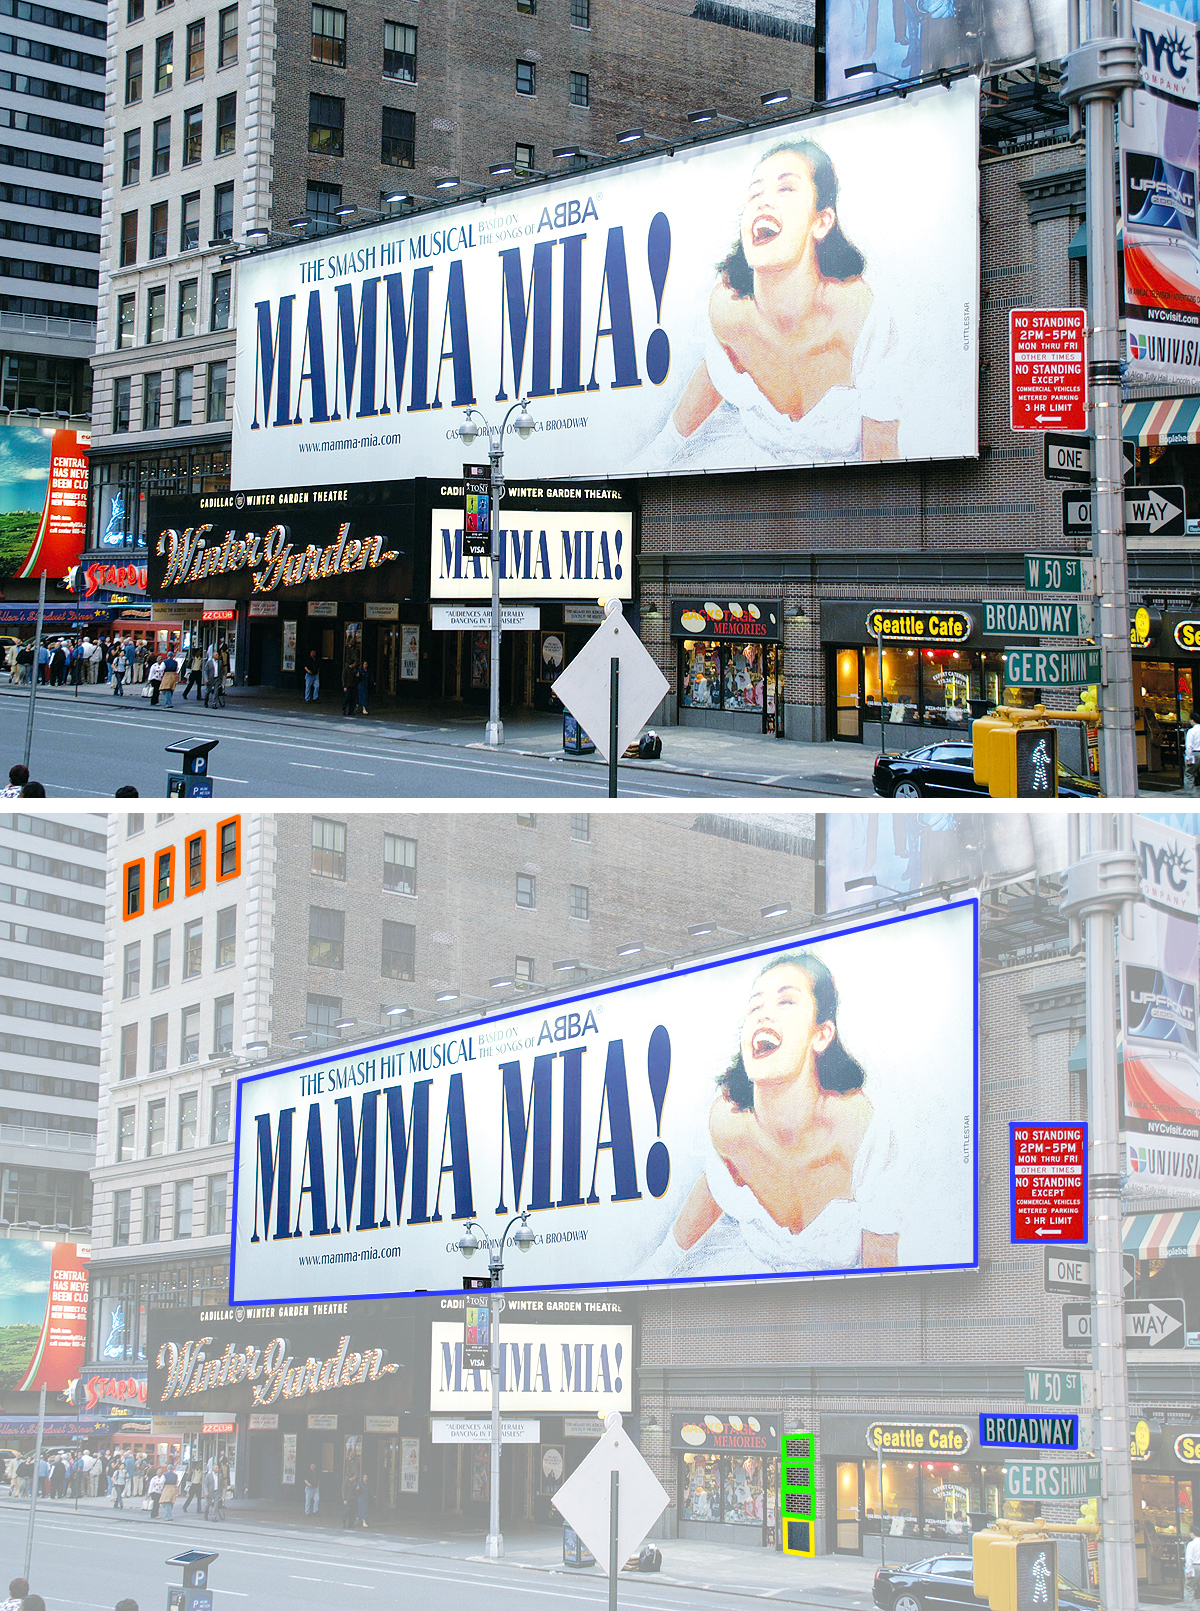
\includegraphics[width=360px]{img/BroadwayPlayers_01_merged.png}
  \caption{An example of rectangle object segmentation in urban environment : Sign plates(blue), windows(red), wall(green), pillar(yellow)}
\label{envexample}
\end{figure}

\newpage
%%%%%%%%%%%%%%%%%%%%%%%%%%%%%%%%%%%%%%%%%%%%%%%%%%%%%%%%%%%%%%%%%%%%%%%%%%%%%%%%%%%%%%%%%%%%%%%%%%%%%%%%%%%%%%%%%%%
%%%%%%%%%%%%%%%%%%%%%%%%%%%%%%%%%%%%%%%%%%%%%%%%%%%%%%%%%%%%%%%%%%%%%%%%%%%%%%%%%%%%%%%%%%%%%%%%%%%%%%%%%%%%%%%%%%%
%%%%%%%%%%%%%%%%%%%%%%%%%%%%%%%%%%%%%%%%%%%%%%%%%%%%%%%%%%%%%%%%%%%%%%%%%%%%%%%%%%%%%%%%%%%%%%%%%%%%%%%%%%%%%%%%%%%
\chapter{사각형 특징의 기하학적 성질을 이용한 스테레오 카메라의 자세 복원 방법}

%\section{렌즈왜곡 모델}
\section{자세 추정을 위한 사각형 복원 방법}
\subsection{평면 Homography를 이용한 카메라의 자세 복원 방법}

종래의 방법으로는 복수의 영상 간 점 특징을 정합하여 자세를 추정한다. 2장의 이미지에 대한 카메라 기하 관계는 epipolar constraint로 표현되며 이를 이용하여 fundamental matrix 또는 essential matrix를 추정하고 두 영상에 대한 카메라 자세 변화를 얻는다. 3개의 이미지에 대해서는 trifocal tensor를 이용하여 카메라 기하관계가 표현된다. 각각의 방법에 대해서는 Nister의 5-point RANSAC 알고리즘\cite{Nister2005}과 Guerrero의 연구\cite{Guerrero2008}가 그 예시이다. 이미지와 카메라간의 n-view geometry에 대해서는 hartley의 저서\cite{Hartley2003}에 보다 상세하게 설명되어 있다.\\
본 논문에서 집중 할 것은 1장의 이미지에 대한 카메라 기하 관계인 homography를 이용하여 카메라의 자세를 추정하는 것이다. Homography는 두 평면 사이의 변환을 표현하는 행렬로, 직사각 특징의 네 점이 한 평면 위에 있다는 가정을 두고 카메라의 자세를 복원한다. 이 접근에서는 2장 이상의 연속된 영상에서 5쌍 이상의 정합된 점을 필요로 하는 기존 방법에 비해 1장의 이미지에서 4개의 점 만으로 유일하게 카메라와 특징간의 상대 자세를 추정할 수 있다는 장점이 있다. \\
일반적인 카메라의 투영을 선형 사상으로 표현한다면 동차좌표계를 이용하여 식 \eqref{homography}과 같이 나타낼 수 있다.

\begin{equation}
\begin{bmatrix} x1'\\x2'\\x3' \end{bmatrix} = \begin{bmatrix} p_{11} & p_{12} & p_{13} & p_{14} \\ p_{21} & p_{22} & p_{23} & p_{24}\\ p_{31} & p_{32} & p_{33} & p_{34} \end{bmatrix}\begin{bmatrix} x1\\x2\\x3\\x4 \end{bmatrix} \label{homography}
\end{equation}

참고로 위의 투영 변환을 모델하기 위해 식 \eqref{pinhole}의 pinhole 카메라 모델을 사용하기도 한다. 이 모델은 렌즈 왜곡에 대한 영향을 무시하고 초점거리, 광축 중심 등의 값으로 이루어진 내부 파라미터 행렬과 카메라의 상대 위치와 자세 정보로 이루어진 외부 파라미터 행렬로 이루어져 있다.

\begin{equation}
s\begin{bmatrix} u\\v\\1 \end{bmatrix} = \begin{bmatrix} f_{x} & s_{skew} & c_{x} \\ 0 & f_{y} & c_{y} \\ 0 & 0 & 1 \end{bmatrix}\begin{bmatrix} r_{11} & r_{12} & r_{13} & t_{X} \\ r_{21} & r_{22} & r_{23} & t_{Y}\\ r_{31} & r_{32} & r_{33} & t_{Z} \end{bmatrix}\begin{bmatrix} X\\Y\\Z\\1 \end{bmatrix} \label{pinhole}
\end{equation}
이는 간단하게 $\mathrm{x}'=K[R|t]\mathrm{x}$로 표현 할 수 있다.
\begin{figure}[!ht]
  \centering
	\includegraphics[width=240px]{img/planar_homography_cropped.pdf}
  \caption{A picture of s same gull looking the other way!}
\label{planar_homography}
\end{figure}
이 때 투영되는 대상이 어떤 평면 위의 점이라면 $Z=0$임을 이용하여 동차좌표계를 위에서 평면 homography 관계를 식\eqref{planar_homography}와 같이 선형방정식으로 표현할 수 있다.

\begin{equation}
\begin{bmatrix} x1'\\x2'\\x3' \end{bmatrix} = \begin{bmatrix} h_{11} & h_{12} & h_{13} \\ h_{21} & h_{22} & h_{23} \\ h_{31} & h_{32} & h_{33} \end{bmatrix}\begin{bmatrix} x1\\x2\\x4 \end{bmatrix} \label{planar_homography}
\end{equation}

이는 간단하게 $\mathrm{x}'=H\mathrm{x}$로 표현 할 수 있고, 이 때 $R=[r_1 \ r_2 \ r_3]$ 이라 하면 $H=K[r_{1} \  r_{2}|t]$이다.
$R$은 정규직교행렬이므로 식 \eqref{rotation_matrix}와 같이 복원할 수 있다.
\begin{equation}
R=\begin{bmatrix}r_1 && r_2 && r_1\times r_2\end{bmatrix} 
\label{rotation_matrix}
\end{equation}

여기서 동차좌표계를 이용한 이와 같은 표현에서 스케일에 대한 정보는 알 수 없으므로 $rank(H)=8$이다. 따라서 두 평면 위의 서로 대응되는 점 쌍으로 평면 homography를 완전하게 추정하기 위해서는 적어도 4개의 쌍이 필요하다. 일반적으로는 카메라의 촬상면에 대응되는 점 만이 직접 측정이 가능하고 실세계의 대응점은 구하기 어려우므로 chessboard를 이용한 카메라 캘리브레이션을 수행할 때와 같이 이미 4개의 점에 대한 형태 정보를 알고 있는 특수한 경우가 아니면 정상적인 자세를 추정할 수 없다.

\subsection{선분 카메라쌍 방법을 이용한 사각형 복원 방법}
본 논문에서는 영상 위의 4개의 점에 대응되는 실세계의 대응 점가질 수 있는 형태 중 직사각형일 경우 가지게 되는 기하적 성질을 이용하여 완전하게 카메라의 자세를 추정하는 방법에 대해 설명한다. 먼저 영상 위의 4개 점을 선분카메라쌍 알고리즘\cite{Lee2012,Lee2013}을 이용하여 원본 사각형의 종횡비를 복원한다. 이 알고리즘은 투영 변환의 불변성인 colinearity를 바탕으로 영상 위의 선분과 실제 선분간의 관계를 Figure \ref{linecamera}와 같은 가상의 선분 카메라 모델로 표현한다. 그러나 하나의 선분카메라만으로는 유일하게 투영 중심을 복원해낼 수 없다. 이에 직사각형을 구성하는 대각선 두 쌍에 대해 선분카메라 모델을 적용할 경우, Figure \ref{coupled_linecamera}와 같이 두 선분카메라의 실제 평면 상 직선의 교차점이 두 직선을 등분하는 점이며 두 선분카메라의 투영중심은 동일하다는 조건을 추가로 이용할 수 있다. 이 조건에 의해 투영변환의 불변성 중 하나인 cross ratio를 이용하여 유일하게 사각형의 종횡비와 그에 대응하는 투영 중심을 복원할 수 있다. Table \ref{CLC_algorithm}에 선분카메라쌍 알고리즘이 기술되어 있다. 복원한 종횡비를 토대로 영상 평면 위 사변형의 꼭지점에 대응되는 실세계 상에서 직사각형의 꼭지점의 좌표를 구성하고 평면 homography를 구해 이전 장의 방법을 이용하여 카메라의 위치와 자세를 추정한다. 이 때 추정되는 위치는 식 \ref{pc_clc}와 같다.
\begin{equation}
\label{pc_clc}
p_c = \frac{d}{\sin\phi}(\cos\theta_0\sin\phi,\ -\cos\theta_0\cos\phi+\cos\theta_1,\ \sin\theta_0\sin\theta_1\sin\rho)
\end{equation}
\\
그러나 선분카메라쌍 기반의 사각형 복원 방법은 원본 사각형의 중점이 정확히 영상의 중심점과 대응되는 특별한 경우에 한하여 적용이 가능하다. 이를 보완하기 위해 소실선의 성질을 이용하여 주어진 사각형에 대해 합동이면서 영상에 대응되는 중심점이 광축에 정렬되는 가상의 사각형을 추출하는 방법이 있다\cite{Lee2014}. 먼저 Figure \ref{offcentered}의 직선 $\overleftrightarrow{w_0 w_1}$을 작도한다. 실세계의 직사각형에 대응되는 두 사변형의 대변을 연장하여 교차점을 찾거나, 별도의 소실점 추정 알고리즘을 사용하여 정렬하고자 하는 사변형에 대응되는 두 개의 소실점을 구한 뒤 직선으로 잇는다. 이렇게 작도한 소실선에서 원본 사변형의 중점과 각 꼭지점을 지나는 직선들과 만나는 두 점을 $w_{d,0}$, $w_{d,1}$이라 할 때, 이 두 점과 영상 중심 $o_m$을 지나는 직선을 작도한다. 원본 사변형의 중심과 영상 중심을 지나는 직선 $\overleftrightarrow{o_m u_m}$이 소실선 $\overleftrightarrow{w_0 w_1}$와 교차하는 점을 $w_m$이라 할 때, 이 점과 원본 사변형의 각 꼭지점을 지나는 직선과 $\overleftrightarrow{w_{d,0} o_m}$, $\overleftrightarrow{w_{d,1} o_m}$ 두 직선들과 이루는 교점을 구하여 중심에 정렬된 사변형을 얻을 수 있다. 이 사변형은 역투영변환 시 원본 사변형에 대응되는 직사각형과 합동인 직사각형을 만들어 내는 성질이 있다. 이는 소실선 위의 점 $w_m$와 사변형의 각 꼭지점을 이은 선분은 원본 직사각형의 스케일변화가 그리는 사각기둥을 두 소실점으로 표현된 투영변환에 의해 영상에 투영된 형태임에 기인한다.
\begin{table}[!t] 
\caption{The coupled line camera algorithm for the rectangle reconstruction}
\label{CLC_algorithm}
\begin{tabular}{p{360pt}}
\toprule[1.5pt]
\textbf{Algorithm} The coupled line camera algorithm for the rectangle reconstruction\\
\hline

\textbf{Input}		$l_i$ - a lenght of line camera, $i=0,1,2,3$.
					$\rho$ - a cross angle of the quadrilateral diagonal.\\
\textbf{Output}		$\phi$ - the crossing angle of rectangle
\\

\hline
\begin{algorithmic}[1]
\For{$i=0,1$}
\State Find division ratio coefficient
\[
\alpha_i = \frac{l_i - l_{i+2}}{l_i + l_{i+2}}.
\]
\EndFor
\State Find relative lenght coefficient
\[
\beta = \frac{l_1}{l_0}.
\]
\State Find lenght of principle axis
\[
d = \sqrt{\frac{(1-\alpha_1)^2\beta^2-(1-\alpha_0)^2}{\alpha_0^2(1-\alpha_1)^2\beta^2-\alpha_1^2(1-\alpha_0)^2}}.
\]
\For{$i=0,1$}
\State Find $\theta_i$ w.r.t
\[
cos\theta_i = d\alpha_i
\]
\EndFor
\State Find $\phi$ w.r.t
\[
	\cos{\phi} = \cos{\theta_0}\cos{\theta_1} + \sin{\theta_0}\sin{\theta_1}\cos{\rho}
\]
\end{algorithmic}\\
\toprule[1.5pt]
\end{tabular}
\end{table}

\newpage

\begin{figure}[!ht]
  \centering
	\includegraphics[width=220px]{img/linecamera_cropped.pdf}
  \caption{The configuration of single line camera model}
\label{linecamera}
\end{figure}
\begin{figure}[!ht]
  \centering
	\includegraphics[width=220px]{img/coupled_linecamera_cropped.pdf}
  \caption{The configuration of coupled line camera model with a rectangle}
\label{coupled_linecamera}
\end{figure}
\newpage
\begin{figure}[!ht]
  \centering
	\includegraphics[width=360px]{img/offcentered_cropped.pdf}
  \caption{Off-Centered quadrilateral alignment with maintaining congruency}
\label{offcentered}
\end{figure}


\newpage

\subsection{3차원 자세 추정을 위한 스테레오 카메라 기반의 선분카메라쌍 방법}
단안 카메라에서 취득한 영상만으로는 3차원 공간 상 특징의 위치를 결정할 수 없다. 이는 투영변환에 의해 스케일에 대한 정보가 손실되기 때문이다. 상기한 선분카메라쌍 알고리즘 및 평면 homography를 이용한 사각형 기반 카메라 자세 추정 방법에서는 실제 크기 대신 중점과 각 꼭지점 간의 거리가 1인 사각형으로 가정한다. 이 경우 같은 장면에서 크기가 다른 복수의 사각형에 대한 위치 추정 결과는 모두 다른 스케일을 가지므로, 동일한 위치에서 촬영된 영상에서 추출한 위치임에도 불구하고 추정에 사용된 특징 별로 상이한 값을 보이게 된다. 이에 스테레오 카메라를 이용하여 특징의 3차원 공간 정보를 완전히 추정하고 한 영상 내부의 복수의 특징에서 추정한 카메라의 위치 및 자세 결과물을 효율적으로 사용하는 방법에 대해 서술한다. \\
스테레오 카메라는 두 pinhole 카메라가 $X$축으로만 $b$만큼의 변위를 가지는 Figure \ref{stereo_triangulation}와 같은 단순한 구조를 가지는 경우로 가정한다. 이 경우 두 카메라에서 3차원상의 점 $P$에 대응하는 점 쌍$X_1=(u_1,v_1)$,$X_2=(u_2,v_2)$에 대해 식 \eqref{stereo}의 관계를 $P$의 위치를 확정할 수 있음을 알 수 있다.
\begin{equation}
\label{stereo}
X=u_1*\frac{Z}{f}, \quad Y=v_1*\frac{Z}{f}, \quad Z=b*\frac{f}{u_1-u_2}
\end{equation}
식 \eqref{stereo}는 왼쪽 카메라를 기준으로 점 $P$의 위치를 표현한 것에 유의한다.\\
선분카메라쌍 알고리즘에서는 중심 정렬된 사각형에 대한 기하적 복원과 위치 추정을 수행한다. 위의 스테레오 카메라를 이용하여 얻을 수 있는 스케일 정보는 Figure \ref{depth_compensate}의 $||\overline{p_c u_m}||$이며 위치 추정 결과의 스케일 보상을 위해 필요한 정보는 직사각형의 중점과 카메라의 투영 중심 사이의 거리 $||\overline{p_c o_m}||$이다. 이는 $o_m$을 중점으로 하는 가상의 정렬된 직사각형을 원점으로 두고 삼각형 $\Delta p_c o_m u_m$에 사인법칙을 적용하여 유도할 수 있다.

Figure \ref{depth_compensate}에서 $||\overline{p_c o_m}||$을 $d$, $||\overline{p_c u_m}||$을 $d'$, 삼각형의 꼭지점인 $p_c$, $o_m$, $v_m$에 대한 각을 $\psi_1$, $\psi_2$, $\psi_3$이라 하고 평면 $\pi$에 대한 법선벡터를 $\overrightarrow{n} = [0 0 1]^T$이라고 둔다. 그 경우 $p_c$의 꼭지각 $\psi_1$는 Figure \ref{linecamera}와 같이 영상평면과 광축이 수직을 이루고, 그 교점을 $u_{om}$이라 할 때 직각삼각형의 성질을 이용하여 아래와 같이 구할 수 있다.

\begin{equation}
\label{angle_psi1}
\psi_1 = \tan^{-1}{\frac{||\overline{u_m u_{om}}||}{f}}
\end{equation}

$o_m$의 꼭지각 $\psi_2$은 평면 $\pi$의 법선벡터와 식 \eqref{pc_clc}를 이용해서 유도할 수 있다.

\begin{equation}
\label{angle_psi2}
\psi_2 = \frac{\pi}{2}-\cos^{-1}\frac{\overrightarrow{n}\cdot\overrightarrow{p_c}}{||\overrightarrow{n}||\ ||\overrightarrow{p_c}||}
\end{equation}

또한 삼각형 $\Delta p_c o_m u_m$에 대해 사인법칙에 의해 아래의 식이 성립한다.
\begin{equation}
\label{sine_rule}
\frac{d'}{\sin\psi_2} = \frac{d}{\sin\psi_3}
\end{equation}
이를 $d$에 대해 정리하면 식 \eqref{depth_compensate_result}와 같다.
\begin{equation}\label{depth_compensate_result}
\begin{split}
d & =\frac{d'}{\sin\psi_2}\sin\psi_3 \\
& =\frac{d'}{\sin\psi_2} \sin(\pi-(\psi_1+\psi_2)) \\
& =\frac{d'}{\sin\psi_2} \sin(\psi_1+\psi_2)
\end{split}
\end{equation}

이와 같이 얻은 $d$를 이용해서 정확한 위치를 얻기 위해 실제 사각형의 크기를 구하여야 한다. Figure \ref{linecamera}에서 직사각형의 중점에서 꼭지점까지 이은 선분에 해당하는 $||\overline{o_m v_0}||$의 거리를 $m$이라고 할 때 $d$와의 관계는 \eqref{rect_size}와 같다.
\begin{equation}
\label{rect_size}
m = d \frac{l_0}{f\sin\theta_0 + l_0\cos\theta_0}
\end{equation}
이를 이용해서 영상 위 원본 사변형의 꼭지점 $u_1$, $u_2$, $u_3$, $u_4$와 중심 정렬 된 직사각형의 꼭지점 $(m,0)$, $(m\cos\phi, m\sin\phi)$, $(-m, 0)$, $(-m\cos\phi, -m\sin\phi)$으로 평면 homography룰 구하여 카메라와 특징 간의 상대 자세를 복원할 수 있다.
\begin{figure}[!ht]
  \centering
	\includegraphics[width=360px]{img/stereo_triangulation_cropped.pdf}
  \caption{The configuration of simple stereo camera model}
\label{stereo_triangulation}
\end{figure}

\begin{figure}[!ht]
  \centering
	\includegraphics[width=360px]{img/depth_compensate_cropped.pdf}
  \caption{Distance compensation for off-centered rectangle}
\label{depth_compensate}
\end{figure}

%%%%%%%%%%%%%%%%%%%%%%%%%%%%%%%%%%%%%%%%%%%%%%%%%%%%%%%%%%%%%%%%%%%%%%%%%%%%%%%%%%%%%%%%%%%%%%%%%%%%%%%%%%%%%%%%%%%
%%%%%%%%%%%%%%%%%%%%%%%%%%%%%%%%%%%%%%%%%%%%%%%%%%%%%%%%%%%%%%%%%%%%%%%%%%%%%%%%%%%%%%%%%%%%%%%%%%%%%%%%%%%%%%%%%%%
%%%%%%%%%%%%%%%%%%%%%%%%%%%%%%%%%%%%%%%%%%%%%%%%%%%%%%%%%%%%%%%%%%%%%%%%%%%%%%%%%%%%%%%%%%%%%%%%%%%%%%%%%%%%%%%%%%%
\chapter{사각형 특징을 이용한 Factor Graph 기반 Visual SLAM}
\section{FactorGraphSLAM}
\cite{Dellaert2006}%Square root SAM
\cite{Kaess2007}%iSAM
\cite{Kaess2011}%iSAM

%%%%%%%%%%%%%%%%%%%%%%%%%%%%%%%%%%%%%%%%%%%%%%%%%%%%%%%%%%%%%%%%%%%%%%%%%%%%%%%%%%%%%%%%%%%%%%%%%%%%%%%%%%%%%%%%%%%
%%%%%%%%%%%%%%%%%%%%%%%%%%%%%%%%%%%%%%%%%%%%%%%%%%%%%%%%%%%%%%%%%%%%%%%%%%%%%%%%%%%%%%%%%%%%%%%%%%%%%%%%%%%%%%%%%%%
%%%%%%%%%%%%%%%%%%%%%%%%%%%%%%%%%%%%%%%%%%%%%%%%%%%%%%%%%%%%%%%%%%%%%%%%%%%%%%%%%%%%%%%%%%%%%%%%%%%%%%%%%%%%%%%%%%%
\chapter{사각형 특징 추출(segmentation)}
%{시각 사각형 특징의 추출 사례}
\cite{Zhang2003}%Extraction, matching and pose recovery based on dominant rectangular structures
\cite{Han2009}%Bottom-up/top-down image parsing with attribute grammar
\cite{Wildenauer2008}%Detection and matching of rectilinear structures
\cite{Jung2004}%Rectangle detection based on a windowed hough transform
\cite{Bazin2007}%Rectangle extraction in catadioptric images
\cite{Bhaskar2010}%Combined spatial and transform domain analysis for rectangle detection

%%%%%%%%%%%%%%%%%%%%%%%%%%%%%%%%%%%%%%%%%%%%%%%%%%%%%%%%%%%%%%%%%%%%%%%%%%%%%%%%%%%%%%%%%%%%%%%%%%%%%%%%%%%%%%%%%%%
%%%%%%%%%%%%%%%%%%%%%%%%%%%%%%%%%%%%%%%%%%%%%%%%%%%%%%%%%%%%%%%%%%%%%%%%%%%%%%%%%%%%%%%%%%%%%%%%%%%%%%%%%%%%%%%%%%%
%%%%%%%%%%%%%%%%%%%%%%%%%%%%%%%%%%%%%%%%%%%%%%%%%%%%%%%%%%%%%%%%%%%%%%%%%%%%%%%%%%%%%%%%%%%%%%%%%%%%%%%%%%%%%%%%%%%
\chapter{사각형 특징을 위한 특징기술자 구조}
%%%%%%%%%%%%%%%%%%%%%%%%%%%%%%%%%%%%%%%%%%%%%%%%%%%%%%%%%%%%%%%%%%%%%%%%%%%%%%%%%%%%%%%%%%%%%%%%%%%%%%%%%%%%%%%%%%%
%%%%%%%%%%%%%%%%%%%%%%%%%%%%%%%%%%%%%%%%%%%%%%%%%%%%%%%%%%%%%%%%%%%%%%%%%%%%%%%%%%%%%%%%%%%%%%%%%%%%%%%%%%%%%%%%%%%
%%%%%%%%%%%%%%%%%%%%%%%%%%%%%%%%%%%%%%%%%%%%%%%%%%%%%%%%%%%%%%%%%%%%%%%%%%%%%%%%%%%%%%%%%%%%%%%%%%%%%%%%%%%%%%%%%%%
\chapter{실험결과}

%%%%%%%%%%%%%%%%%%%%%%%%%%%%%%%%%%%%%%%%%%%%%%%%%%%%%%%%%%%%%%%%%%%%%%%%%%%%%%%%%%%%%%%%%%%%%%%%%%%%%%%%%%%%%%%%%%%
% set second argument of \begin to the number of references
% (used to reserve space for the reference number labels box)

\bibliographystyle{IEEEtran}%...는 bst 파일의 이름(확장자 없이)
\bibliography{ThesisBibTeX.bib}%...는 bib 파일의 이름(확장자 없이)
%\begin{thebibliography}{1}
%\bibitem{greenberg}
%A. Greenberg, J. Hamilton, D.A. Maltz, and P. Patel,
%\emph{The cost of a Cloud: Research Problems in Data Center Networks},
%ACM SIGCOMM Computer Communication Review (CCR), 
%Vol. 39, No. 1, pp. 68-73, January 2009.
%
%\bibitem{wallin}
%S. Wallin, V. Leijon, 
%\emph{Telecom Network and Service Management: An Operator Survey}, 
%MMNS, 2009.
%
%\bibitem{hscalability}
%Wikipedia, \emph{Horizontal Scalability},
%\url{http://en.wikipedia.org/wiki/Scalability#Scale_horizontally_.28scale_out.29}
%
%\end{thebibliography}


\chapter*{감사의 글}

감사의 글을 적으시면 되겠습니다.
감사합니다.

\begin{flushright}
\vspace{1cm}
이재민 배상
\end{flushright}

\end{document}


